\documentclass{beamer}

\usefonttheme{professionalfonts} % using non standard fonts for beamer
\usefonttheme{serif} % default family is serif

\usepackage{enumitem}
\setitemize{label=\usebeamerfont*{itemize item}%
  \usebeamercolor[fg]{itemize item}
  \usebeamertemplate{itemize item}}

\usepackage{hyperref}
%\usepackage{minted}
\usepackage{animate}
\usepackage{graphicx}
\def\Put(#1,#2)#3{\leavevmode\makebox(0,0){\put(#1,#2){#3}}}
\usepackage{colortbl}
\usepackage{tikz}
\usepackage{amssymb}
\usepackage{enumerate}
\usepackage{arydshln}
\usepackage{algorithm}
\usepackage{algpseudocode}

\colorlet{lightred}{red!25}
\colorlet{lightgreen}{green!25}
\beamertemplatenavigationsymbolsempty

\newcommand\blfootnote[1]{%
  \begingroup
  \renewcommand\thefootnote{}\footnote{#1}%
  \addtocounter{footnote}{-1}%
  \endgroup
}

\makeatletter

%% Textclass specific LaTeX commands.
\newcommand\makebeamertitle{\frame{\maketitle}}%
\AtBeginDocument{%
  \let\origtableofcontents=\tableofcontents
  \def\tableofcontents{\@ifnextchar[{\origtableofcontents}{\gobbletableofcontents}}
  \def\gobbletableofcontents#1{\origtableofcontents}
}
%% User specified LaTeX commands.
\usetheme{Malmoe}
\useoutertheme{infolines}
\addtobeamertemplate{headline}{}{\vskip2pt}
\setbeamercovered{transparent}

\makeatother

%%%%%%%%%%%%%%%%%%%%%%%%%%%%%%%%%%%%%%
%% Main document
%%%%%%%%%%%%%%%%%%%%%%%%%%%%%%%%%%%%%%
\begin{document}
\title[PFLOCK report]{PFLOCK Report}
\author[AC]{Andres Calderon}
\institute[Fall'20]{University of California, Riverside}
\makebeamertitle
\newif\iflattersubsect

\AtBeginSection[] {
    \begin{frame}<beamer>
    \frametitle{Outline} 
    \tableofcontents[currentsection]  
    \end{frame}
    \lattersubsectfalse
}

\AtBeginSubsection[] {
    \begin{frame}<beamer>
    \frametitle{Outline} 
    \tableofcontents[currentsubsection]  
    \end{frame}
}

\begin{frame}{Sample cliques...}
    \begin{minipage}[t]{0.48\textwidth}
        3 15 11 13 6 1 5 7 12 4 14 9 8 10 2 \\
        3 15 11 13 6 1 5 7 12 4 14 9 16 17 \\
        3 15 11 13 6 1 5 7 12 4 14 9 16 8 \\
        3 15 11 13 6 1 5 7 12 4 14 16 17 18 \\
    \end{minipage}
    \begin{minipage}[t]{0.48\textwidth}
        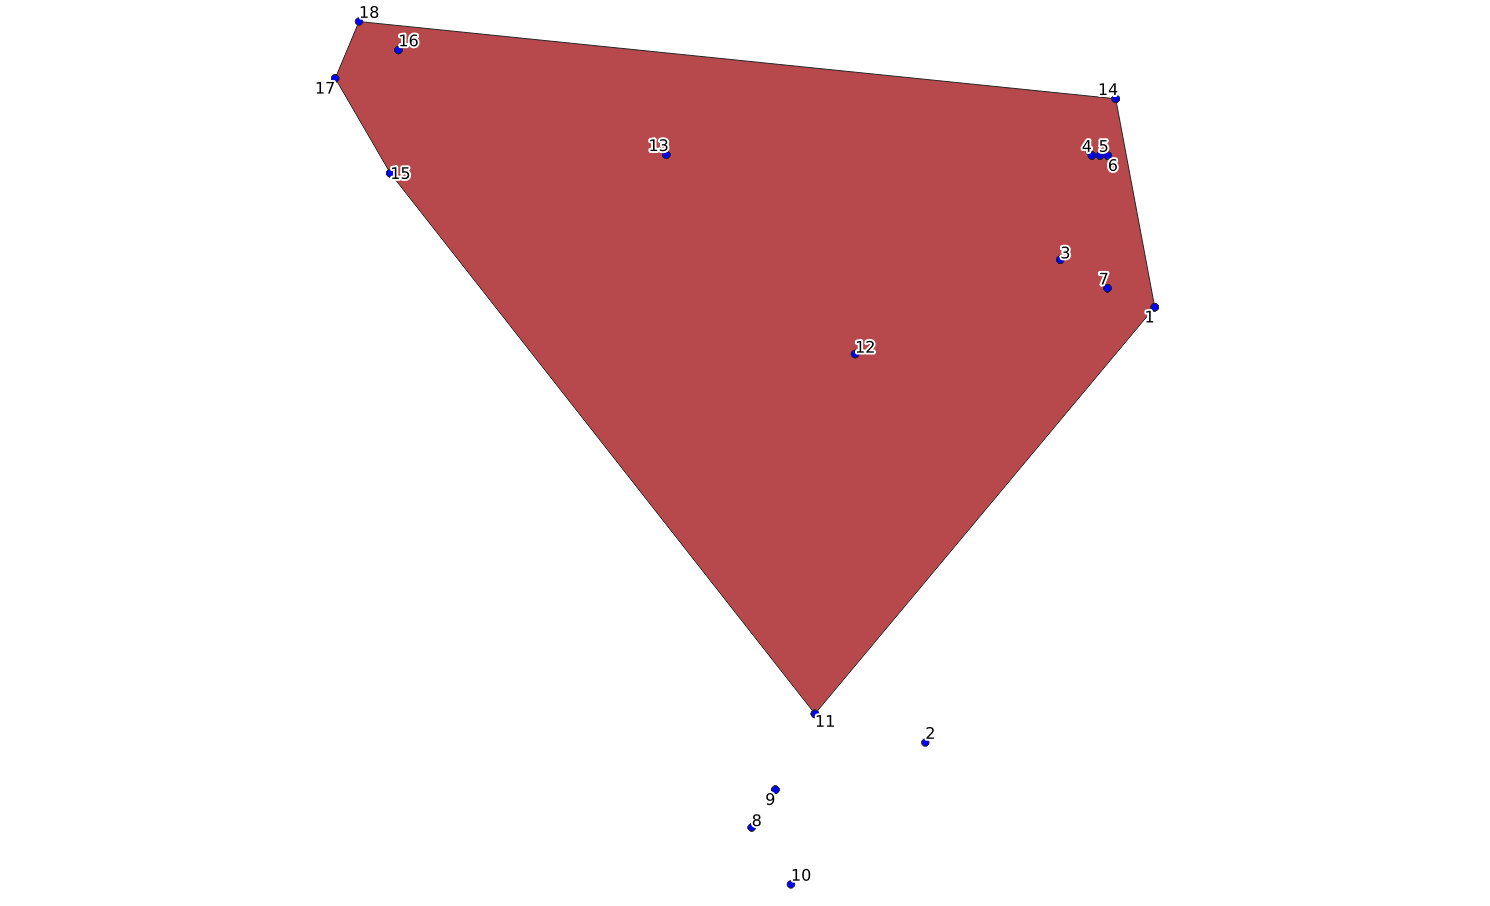
\includegraphics[trim=220 0 250 0,clip,width=\textwidth]{figures/cliques}
    \end{minipage}
\end{frame}

\begin{frame}{Prefixtree...}
    \centering
    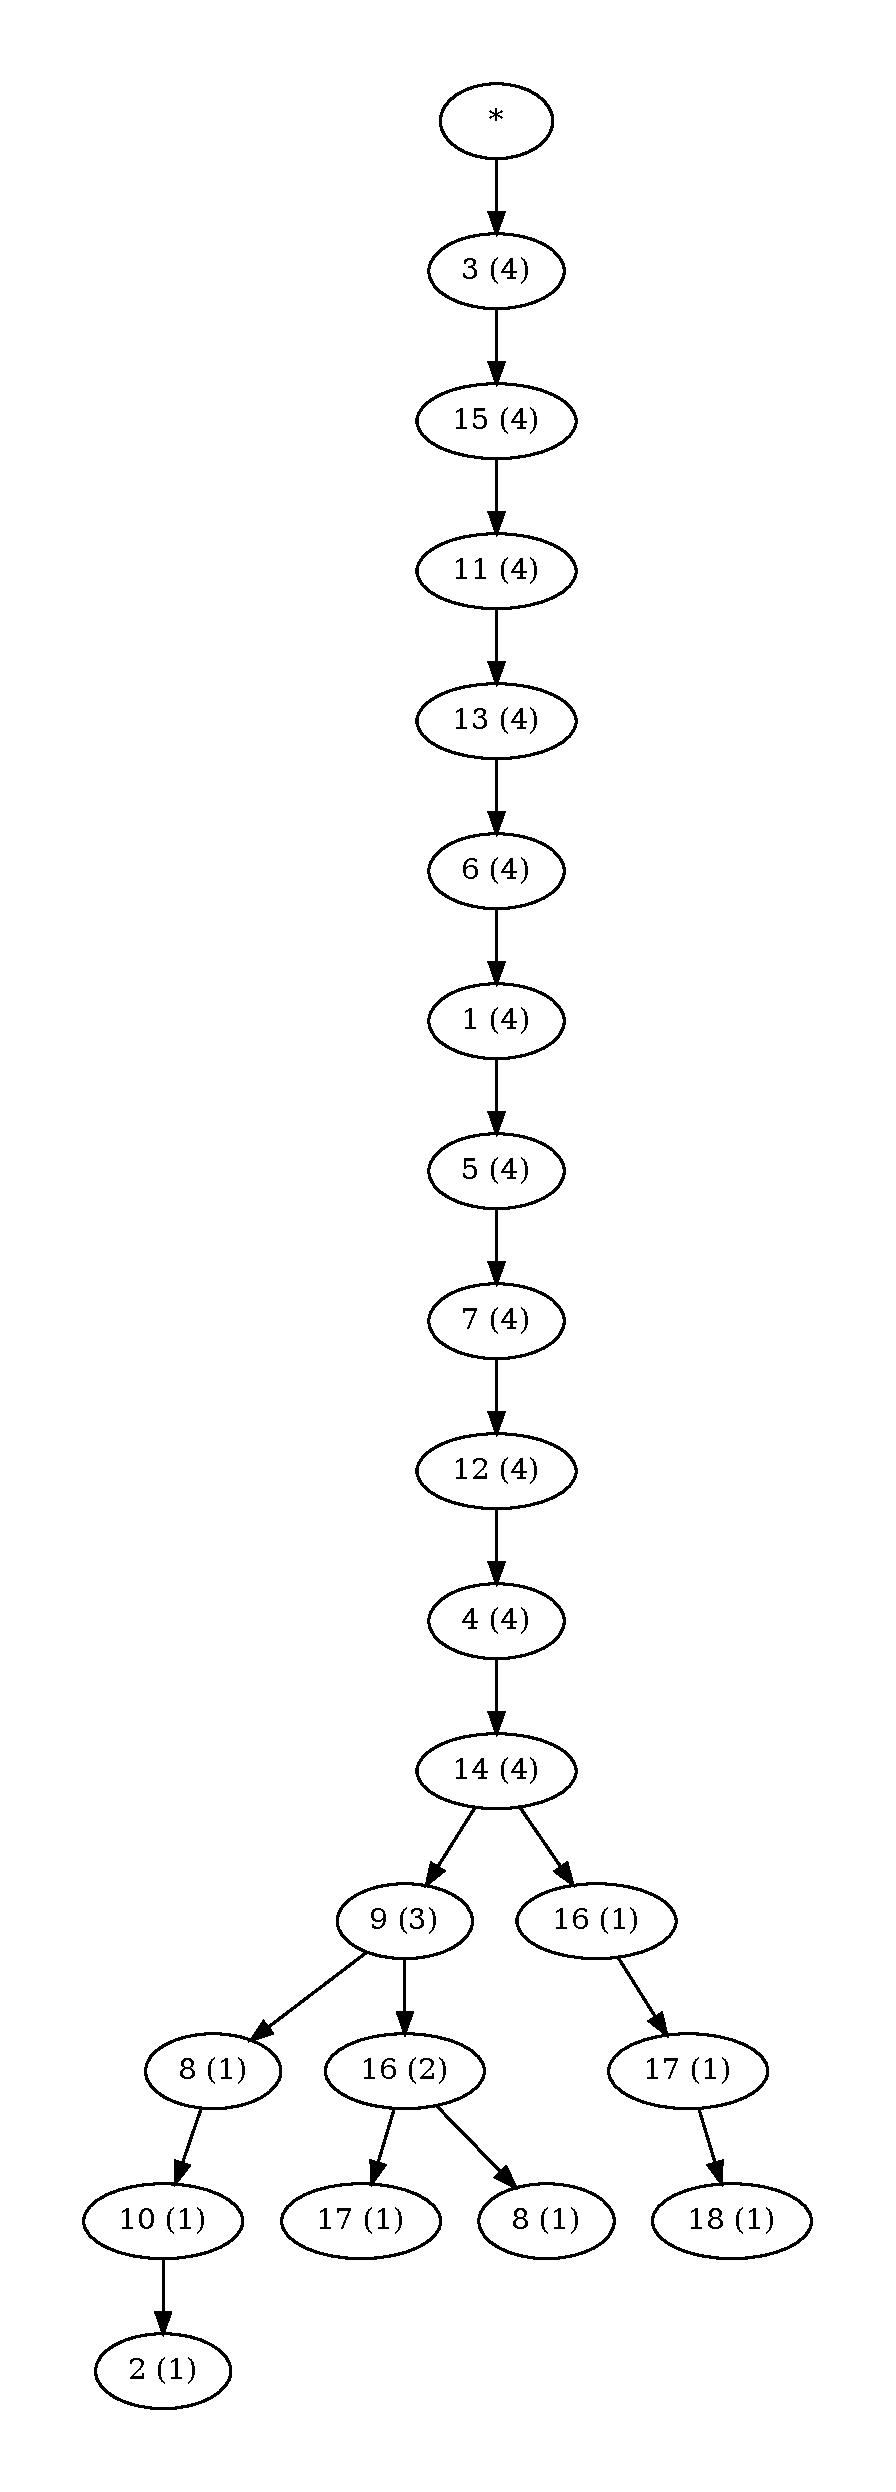
\includegraphics[width=0.245\textwidth]{figures/prefixtree}
\end{frame}

\begin{frame}{Algorithm...}
        0. Find first node with more than one branch. \\
        1. Compute initial set of Candidates and Flocks for that node. \\
        2. For each subsequent node: \\
            \hspace{1cm} 2.1 If $point \bigcap Flocks$: \\
            \hspace{2cm} add point to those flocks. \\
            \hspace{1cm} 2.2 If $point \bigcap Candidates$: \\
            \hspace{2cm} add point to those candidates. \\
            \hspace{2cm} if $candidate.size >= \mu$: \\
            \hspace{3cm} move candidate to flocks. \\
        3. Collect flocks at each leaf. \\
        4. Prune duplicates. \\
\end{frame}
\end{document}

